\documentclass{beamer}
\usetheme{Madrid}

\usepackage[ngerman,english]{babel}
\usepackage[utf8]{inputenc}
\usepackage[T1]{fontenc}
\usepackage{siunitx}
\usepackage{lmodern}
\usepackage{subfigure}
\usepackage{multirow}
\usepackage{caption}
\usepackage{graphicx}
\usepackage{cite}



\begin{document}

\title[HF-Chirurgie]{Hochfrequenzchirurgie}
\author{H. Merk}
\date{\today}

\begin{frame}
\maketitle
\end{frame}


\begin{frame}
\frametitle{Inhalt}
\tableofcontents
\end{frame}



\section{Einleitung}
\begin{frame}
\frametitle{Einleitung}
	\begin{block}{Was ist HF-Chirurgie?}
		Unter der Hochfrequenzchirurgie versteht man den assistierenden Einsatz von elektrischer Energie in der Chirurgie zur thermisch induzierten Veränderung oder Zerstörung von Gewebezellen mit dem Ziel der Hämostase (Blutstillung), Gewebedurchtrennung oder -versiegelung \cite{kramme2016medizintechnik}.
	\end{block}
	\begin{minipage}[t]{0.49\textwidth}
		\only<2->{
		\vspace{1cm}
		\textbf{Drei essentielle Bauteile:}
		\begin{itemize}
			\item Hochfrequenzgenerator
			\item Erdung
			\item Handstück mit Applikator
		\end{itemize}}
	\end{minipage}
	\begin{minipage}[t]{0.49\textwidth}
		\only<2->{
		\vspace{0cm}
		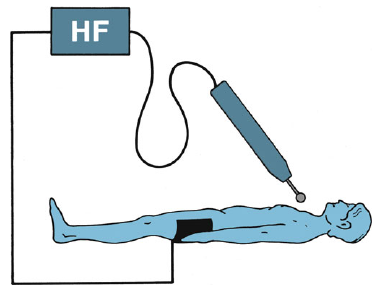
\includegraphics[height=4cm]{images/monopolareTechnik.png}}
	\end{minipage}
\end{frame}


\section{Grundlagen}
\begin{frame}
\frametitle{Grundlagen}
\framesubtitle{Elektrische Wechselwirkung mit dem Gewebe}
\textbf{Elektrische Wechselwirkung ist frequenzabhängig:}
\vspace{0.5cm}
\begin{itemize}
	\item Gleichstrom ($f=\SI{0}{\hertz}$): \emph{elektrolytische Wirkung} \\$\rightarrow$ Ionenverschiebung/elektrochemische Prozesse
	\vspace{0.2cm}
	\item Wechselstrom ($f=\SI{20}{\hertz}-\SI{20}{\kilo\hertz}$): \emph{faradische Effekte}
	\\$\rightarrow$ Störung der Nerven- \& Muskelreizung, insbesondere des Herzens
	\vspace{0.2cm}
	\item Wechselstrom ($f>=\SI{300}{\kilo\hertz}$): \emph{thermische Effekte}
	\\$\rightarrow$ effektive Energieübertragung auf das Gewebe
	\\$\rightarrow$ hohe Frequenzen = hohe Leitfähigkeit im Gewebe, das vor allem einen kapazitiven Widerstand hat (Zellen)
\end{itemize}
\end{frame}



\begin{frame}
\frametitle{Grundlagen}
\framesubtitle{Thermische Prozesse im Gewebe}
\textbf{Gewebestrukturänderung aufgrund Temperaturerhöhung:}
	\begin{itemize}
		\item $37^\circ-45^\circ$ $\rightarrow$ \emph{Erwärmung} des Gewebes
		\item $45^\circ-70^\circ$ $\rightarrow$ \emph{Proteindenaturierung} (3D-Struktur der Proteine geht verloren, d.h. auch ihre Funktion)
		\item $70^\circ-100^\circ$ $\rightarrow$ \emph{Koagulation} (Verklumpen von Proteinen)
		\item $100^\circ-300^\circ$ $\rightarrow$ \emph{Karbonisation} (Gewebe trocknet aus)
		\item über $300^\circ$ $\rightarrow$ \emph{Verdampfen und Abtragung} des Gewebes
	\end{itemize}
	\begin{figure}
		\centering
		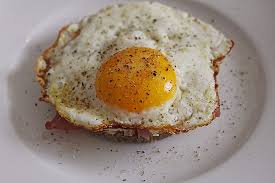
\includegraphics[width=4cm]{images/spiegelei.png}
	\end{figure}
\end{frame}


\begin{frame}
\frametitle{Grundlagen}
\framesubtitle{Parameterabhängigkeit}
\begin{center}
	Erwärmung des Gewebes ist abhängig von der:
\end{center}
\begin{enumerate}
	\item \textbf{Stromdichte}: $S=\frac{I}{A}$
	\\$\rightarrow$ Strom $I$ hängt ab vom spez. Widerstand des Gewebes \& verwendete Effektivspannung $U_{effektiv}=R_{Gewebe}\cdot I$
	\vspace{0.5cm}
	\item \textbf{Einwirkzeit}: Elektrische Energie wird in Wärme umgewandelt
	\\$\rightarrow$ je länger der Wärmefluss ins Gewebe, desto höher der Temperaturanstieg.
\end{enumerate}
\end{frame}


\begin{frame}
\frametitle{Grundlagen}
\framesubtitle{Schneiden und Koagulation}
	Zwei grundlegende Effekte in der HF-Chirurgie:
	\vspace{0.5cm}
	\begin{enumerate}
		\item \textbf{Schneiden}: Verdampfung \& Ionisierung des Wassergehaltes
		\\$\rightarrow$ Sinuswelle führt zu extremen Spitzen des Temperaturanstiegs
		\vspace{0.1cm}
		\item \textbf{Koagulieren}: thermische Denaturierung des Gewebes
		\\$\rightarrow$ diskontinuierliche Wellenpakete mit Ruhephasen lassen Gewebe abkühlen
	\end{enumerate}
	\begin{figure}
	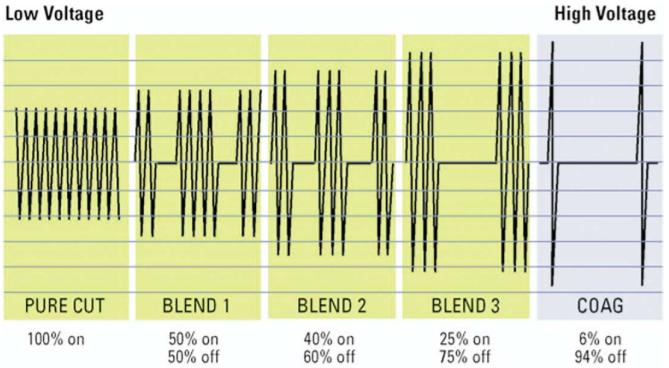
\includegraphics[width=4.5cm]{images/_stromModi.png}
	\hspace{0.5cm}
	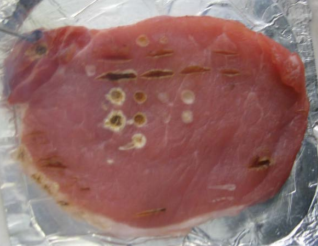
\includegraphics[width=2.85cm]{images/fleisch.png}
	\cite{stromModi}
	\end{figure}
\end{frame}



\section{Anwendung}
\begin{frame}
\frametitle{Anwendung}
\framesubtitle{Bipolare Technik}
	\begin{center}
		Für die Erzeugung eines elektrischen Stromes benötigt man zwei Elektroden.
	\end{center}
	\textbf{Bipolare Technik:}
	Applikator besitzt zwei Spitzen (Pinzette), zwischen denen die Spannung anliegt. Gewebe wird zwischen Pinzettenspitzen genommen. \\\textcolor{red}{$\Rightarrow$ Stromfluss}
	\begin{figure}
		\centering
		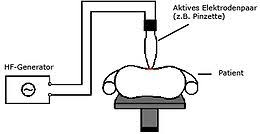
\includegraphics[width=6cm]{images/_bipolareTechnik.png}
		\cite{wiki:HF}
	\end{figure}
\end{frame}


\begin{frame}
\frametitle{Anwendung}
\framesubtitle{Monopolare Technik}
	\textbf{Monopolare Technik:}
	Strom fließt zwischen Applikatorelektrode und großflächiger Gegenelektrode. Die Stromdichte an der Applikatorelektrode ist sehr hoch
	\\\textcolor{red}{$\Rightarrow$ thermische Effekte}
	\begin{figure}
		\centering
		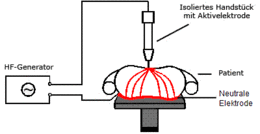
\includegraphics[width=6cm]{images/_monopolareTechnik.png}
		\cite{wiki:HF}
	\end{figure}
	\begin{itemize}
		\item E-Feld-Linien fächern sich außerhalb des WW-Volumens auf \\$\rightarrow$ Stromdichte unkritisch
		\item Gewissenhafte Aubfbringung der Gegenelektrode
		\item keine Berührung durch dritte Personen
	\end{itemize}

\end{frame}


\begin{frame}
\frametitle{Weiterführende Anwendungen}
\framesubtitle{Argonassistiertes Schneiden}
\begin{itemize}
	\item Nutzung eines Schutzgases (Argon) während der HF-Anwendung:
	\begin{itemize}
		\item [$\rightarrow$]Verdrängung des Luftsauerstoffes aus dem WW-Volumen
		\item [$\rightarrow$]Reduzierung der Karbonisierung
		\item [$\rightarrow$]Verbesserung der Sicht des Operateurs aufgrund minimierter Rauchbildung
	\end{itemize}
	\vspace{0.2cm}
	\item Anwendungsgebiete: 
	\begin{itemize}
		\item [$\rightarrow$] Dermatologie
		\item [$\rightarrow$] allgemeine Weichteilchirurgie
	\end{itemize}
\end{itemize}
\begin{figure}
	\centering
	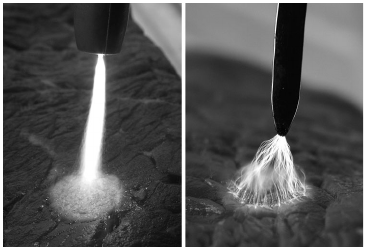
\includegraphics[width=4.5cm]{images/argon.png}
	\cite{kramme2016medizintechnik}
\end{figure}
\end{frame}



\begin{frame}
\frametitle{Weiterführende Anwendungen}
\framesubtitle{Piezo-Chirurgie zur Hartgewebebearbeitung}
	\begin{itemize}
		\item HF-Chirurgie für Hartgewebe (Knochen,Knorpel) nicht geeignet, da die Leitfähigkeit zu gering ist $\Rightarrow I=\frac{U_{effektiv}}{R_{Gewebe}}$
		\item \textbf{Piezo-Chirurgie:} Piezo-Kristalle ändern bei angelegter Spannung ihre Länge\\
		\textcolor{red}{$\Rightarrow$ kleine Längenänderung ($\approx\mu m$) bei hohen Frequenzen ($\SI{25}{\kilo\hertz}-\SI{30}{\kilo\hertz}$)}	
		\item gleichzeitige Schonung von Weichgewebe, da das Weichgewebe der kleinen Oszillation nicht folgen kann und somit nicht beschädigt wird
		\item Anwendung und Vorteile:
		\begin{itemize}
			\item Mund-Kiefer-Gesichtschirurgie (z.B Präparation des Kieferknochens bei Schonung des \emph{nervus facialis})
			\item preiswert
			\item verschiedene Applikatoren
			\item Handhabung ähnlich zu gängigen Methoden
		\end{itemize}
	\end{itemize}
\end{frame}


\begin{frame}{Piezo-Chirurgie}
\framesubtitle{Clip}
\begin{figure}
	\centering
	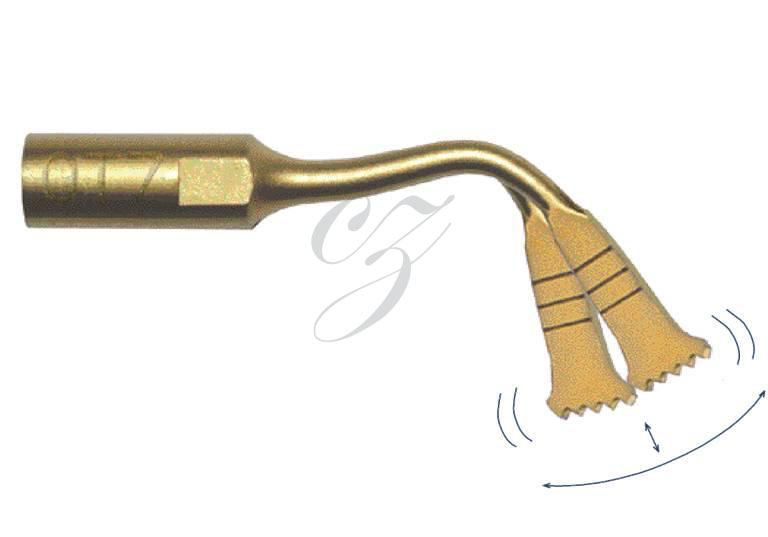
\includegraphics[width=5cm]{images/piezoChirurgie.png}
\end{figure}
\end{frame}


\section{Zusammenfassung}
\begin{frame}
\frametitle{Zusammenfassung}
	\begin{itemize}
		\item HF-Chirurgie nutzt elektrische Energie zur thermischen Veränderung/Zerstörung von Gewebezellen
		\begin{itemize}
			\item [$\rightarrow$]Blutstillung
			\item [$\rightarrow$]Gewebedurchtrennung/-versiegelung
		\end{itemize}
		\item Essentielle Bauteile: Hochfrequenzgenerator, Erdung, Handstück mit Applikator
		\item Wechselstrom ($f>=\SI{300}{\kilo\hertz}$) wird benutzt um thermische Effekte im Gewebe zu verursachen:
		\begin{itemize}
			\item $70^\circ-100^\circ$ $\rightarrow$ \emph{Koagulation} (Verklumpen von Proteinen)
			\begin{itemize}
				\item [$\rightarrow$]thermische Denaturierung des Gewebes
			\end{itemize}
			\item über $300^\circ$ $\rightarrow$ \emph{Verdampfen und Abtragung} des Gewebes zum Schneiden
			\begin{itemize}
				\item [$\rightarrow$]Verdampfung \& Ionisierung des Wassergehaltes
			\end{itemize}
		\end{itemize}
	\end{itemize}
\end{frame}


\begin{frame}
\frametitle{Zusammenfassung}
	\begin{itemize}
		\item Bipolare Technik:	Applikator besitzt zwei Spitzen (Pinzette), zwischen denen die Spannung anliegt. Gewebe wird zwischen Pinzettenspitzen genommen.
		\item Monopolare Technik: Strom fließt zwischen Applikatorelektrode und großflächiger Gegenelektrode. Die Stromdichte an der Applikatorelektrode ist sehr hoch.\\
		$\rightarrow$ E-Feld-Linien fächern sich außerhalb des Wechselwirkungsvolumens auf $\rightarrow$ Stromdichte unkritisch 
	\end{itemize}
\textcolor{red}{$\Rightarrow$ Stromkreis geschlossen}\\
\textcolor{red}{$\Rightarrow$ Schneiden oder Koalugieren mithilfe thermischer Effekte}
	\begin{figure}
	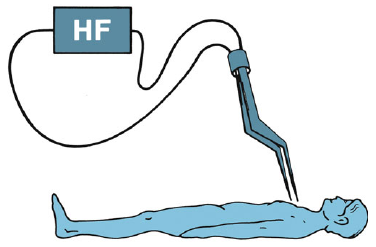
\includegraphics[width=2.8cm]{images/bipolareTechnik.png}
	\hspace{1cm}
	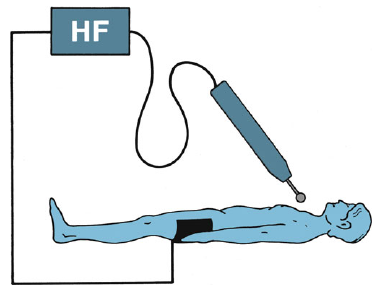
\includegraphics[width=2.5cm]{images/monopolareTechnik.png}
	\end{figure}
\end{frame}


\section{Ausblick}
\begin{frame}
\frametitle{Ausblick}
	\begin{itemize}
		\item Doppelseitiges Handstück \cite{dual}
		\begin{itemize}
			\item automatisches Wechseln mit einer simplen Handbewegung\\
			$\rightarrow$ hastiges Wechseln der Applikatoren wird vermieden		
		\end{itemize}
		\begin{figure}
			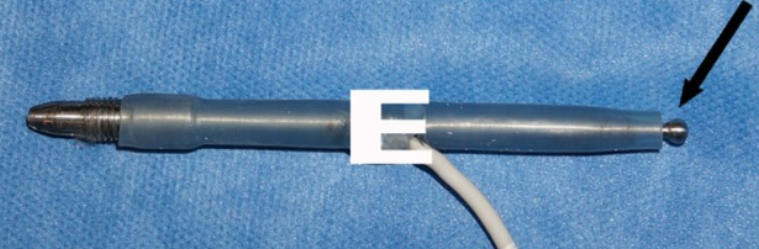
\includegraphics[width=2.8cm]{images/dual.png}
		\end{figure}
		\item drahtloser Fußschalter (auf Bluetooth-Basis) als Alternative zu den bisherigen Knöpfen am Handstück \cite{kramme2016medizintechnik}
		\begin{itemize}
			\item Wirtschaftlichkeit muss sich beweisen (Kosten/Nutzen-Faktor)
		\end{itemize}
		\item wasserkühlendes System \cite{waterCool}
		\begin{itemize}
			\item spezielle Handgriffkonfiguration
			\item Kühlmittel strömt von der Applikatorspitze zur Gewebeschnittstelle\\
			$\rightarrow$ Reduktion der Gewebewärme zur Minderung des Gewebeschadens\\
			$\rightarrow$ Experimentelle Ergebnisse: Reduktion um $100\mu m$ an Schichtdicke
		\end{itemize}
		\begin{figure}
			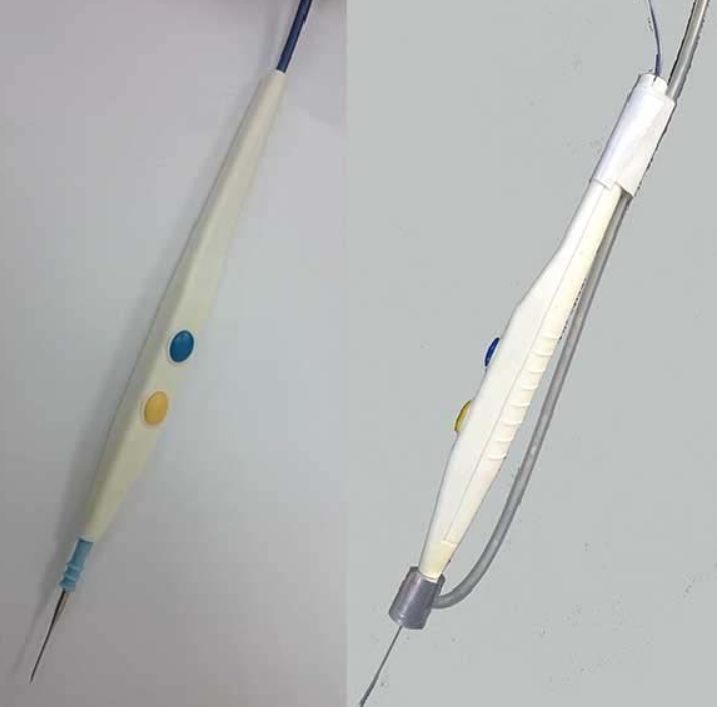
\includegraphics[width=1.8cm]{images/waterCool.png}
		\end{figure}
	\end{itemize}
\end{frame}


\begin{frame}[shrink]
\frametitle{Quellenangabe}
	\bibliographystyle{unsrt}
	\bibliography{Literatur}
\end{frame}

%__________________________________________________________
\begin{frame}
\centering
\textbf{Vielen Dank für eure Aufmerksamkeit}
\end{frame}

\end{document}